% 必要な項目ができた場合は適宜サブセクションを追加してください

%\include{begin}
\documentclass[a4j,titlepage]{jarticle}
\usepackage[dvipdfmx]{graphicx,epsfig}

\usepackage{longtable}

\usepackage{textcomp}



\usepackage{float}

\usepackage{ascmac}
\usepackage{fancybox}
\usepackage{url}


\begin{document}

% イベント名を記入する
\section{アイスブレイキング}


% 日時と場所を記入する
% 時刻は4桁で記入すること!
\subsection{日時・場所}
\begin{tabular}{p{2zw}rp{38zw}}
  日時 & : & 2019年4月6日(土) 09:00 $\sim$ 09:40\\
  場所 & : & つどいの広場
\end{tabular}


% 目的を記入する
\subsection{目的}
  本イベントでは,「ワードウルフ」というゲームを通して打ち解け合い,楽しく話し合う環境を作ることで,これからのスケジュールを楽しんでもらうことを目的とする.

% イベントの概要やルールを記入する
\subsection{イベント内容}
  ワードウルフは制限時間内でグループの中での少数派の人を探すゲームである.自分が多数派か少数派かわからない状況でグループ内で話し合い,少数派と多数派の意見のズレを探して誰が少数派かを予測する.自分が少数派だと思ったら少数派だと知られないように多数派になりすまし,上手く立ち振る舞う.

% イベントのタイムスケジュールを記入する
% 時刻は必ず4桁(00:00)で記入すること!
% 時間の流れは途切れないように記述する!
\subsection{タイムスケジュール}
\begin{longtable}{p{3zw}p{39zw}}
  09:00 & \textbf{◎ 整列} \\
        & \ \  各スタッフは新入生と教員方を誘導して整列する. 整列完了後,その場に座る.(図\ref{fig:ice}を参照) \\
        & \ \  次の仕事を控えたスタッフは準備に入る. \\
        & \ \  整列を終え,全員が座ったら頃合いを見て司会は話し始める.\\

  09:03 & \textbf{◎ アイスブレイクの説明}\\
        & \ \  パワーポイントを用いてアイスブレイクの説明を行う.\\
        & \ \  分からない新入生がいたら各班のスタッフが補足説明を行う.\\
        & \ \  スタッフから順番に自己紹介をしていく(名前,出身県,100万あったら何したい). \\

  09:10 & \textbf{◎ ワードウルフの説明}\\
        & \ \  パワーポイントを用いてワードウルフの説明を行う.\\
        & \ \  分からない新入生がいたら各班のスタッフが補足説明を行う.\\

  09:14 & \textbf{◎ ワードウルフの開始}\\
        & \ \  スタッフがお題の紙を配る.\\
        & \ \  プレゼンターが時間を計り,7分間話し合って少数派を見つける.\\
        & \ \  その後,自分のお題の紙を全員で見せ合い,答え合わせをする.\\

  09:25 & \textbf{◎ アイスブレイキング終了し休憩(10分間)}\\

\end{longtable}


% イベントに必要な役割と人数を記入する
% 担当者は決定次第追記する
% 記入例 ・司会者 2人(名前1、名前2)
\subsection{人員配置}
\begin{itemize}
\item 司会:横田,長通
\item プレゼンター:藤沢,堀川
\item プラカード:各班スタッフ代表
\end{itemize}


% イベントを実施するときに新入生や先生、スタッフがどこに配置するかを記入する
% 図があるとわかりやすい
\subsection{全体配置}
\begin{figure}[h]
  \begin{center}
    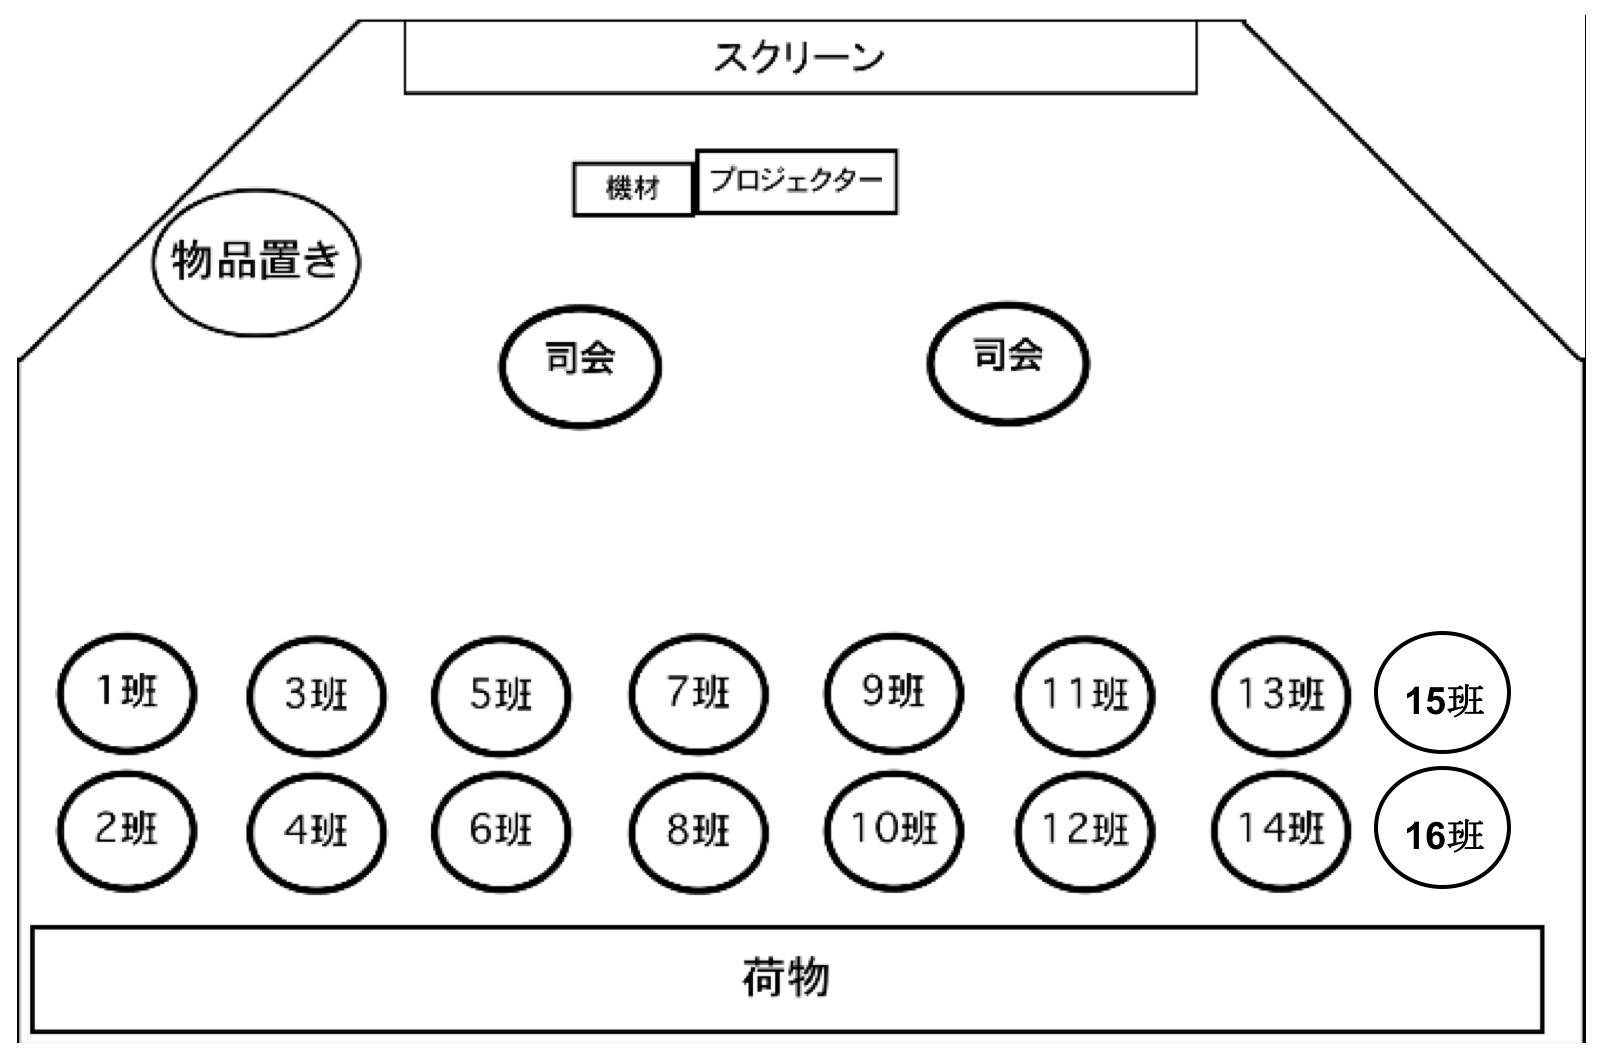
\includegraphics[scale=0.5]{./21/ice.eps}
    \caption{アイスブレイクの全体配置}
    \label{fig:ice}
  \end{center}
\end{figure}


% イベントに必要な物品と個数を記入する
% 記入例 ・マジックペン 10本
\subsection{必要物品}
\begin{itemize}
\item マイク(司会用)3本
\item スピーカー 2台
\item プロジェクタ 1台
\item 長机(プロジェクタ設置用) 1台
\item 椅子(機器操作用) 1脚
\item スクリーン 1台
\item ノートパソコン 1台
\item お題が書かれた紙(10枚程度)が入った封筒 16班1セット
\end{itemize}


% 注意事項やスタッフに周知しておくべきことがあれば記入する
\subsection{備考}
時間が短いので手早い行動を心掛けて下さい.

%\include{end}

\end{document}
